\newpage
\section{Geometry and Multiplying Complex Numbers}\label{A:complexMultiplication}
\fixnote{Maybe simplify Louie further.  Make tables for calculation.  Then summarize the results in another table.}  


Now we'll investigate the geometry of multiplying complex
numbers. In each case, specify the transformation.  For example, if you see a rotation, specify the angle and the center of rotation.  

Louie Llama\index{Louie Llama} is here to help us out:
\[
\begin{tabular}{ccc}

\includegraphics[scale=.5]{../graphics/llama.pdf} & \qquad $\leftrightsquigarrow$\qquad& 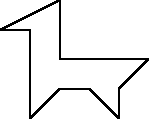
\includegraphics{../graphics/llamaPlot.pdf}\\
Louie Llama & & how we'll draw him
\end{tabular}
\]

\begin{prob} 
Here's Louie Llama hanging out near the point $0$ in the complex
plane. Multiply him by $2$. Make a table and show in the plane below what happens.  What transformation do you see?  
\[
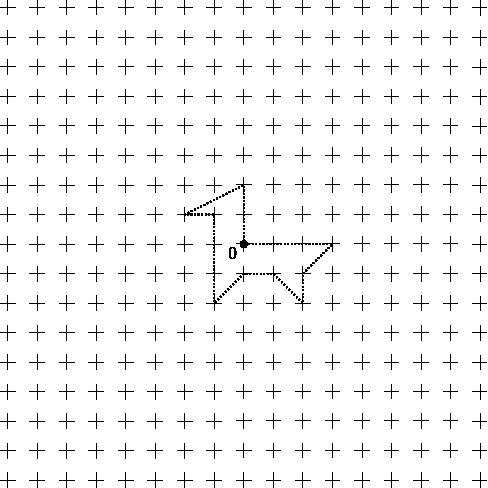
\includegraphics{../graphics/complexMult.pdf}
\]
\end{prob}

\break

\begin{prob} 
Now multiply him by $i$. Make a table and show in the plane below what happens.  What transformation do you see?  
\[

\includegraphics{../graphics/complexPlane.pdf}
\]
\end{prob}

\vfill

\begin{prob} 
Now multiply Louie Llama by $1+i$. Make a table and show in the plane
below what happens.  What transformation do you see?  
\[

\includegraphics{../graphics/complexPlane.pdf}
\]
\end{prob}

\vfill



\begin{prob} 
Now multiply Louie Llama by $\frac{1}{2}+\frac{\sqrt{3}}{2}i$. Make a
table and show in the plane below what happens.  What transformation do you see?  
\[

\includegraphics{../graphics/complexPlane.pdf}
\]
\end{prob}


\begin{prob} 
Geometrically speaking, what does it mean to ``multiply'' complex
numbers?
\end{prob}



\begin{prob}
Summarize your results from the previous problems.  
Then explain what happens when we ``multiply'' Louie Llama by a complex
number. 
\end{prob}
